%!TEX TS-program = xelatex
\documentclass[]{friggeri-cv}
\usepackage{afterpage}
\usepackage{hyperref}
\usepackage{color}
\usepackage{xcolor}
\usepackage{smartdiagram}
\usepackage{fontspec}
% if you want to add fontawesome package
% you need to compile the tex file with LuaLaTeX
% References:
%   http://texdoc.net/texmf-dist/doc/latex/fontawesome/fontawesome.pdf
%   https://www.ctan.org/tex-archive/fonts/fontawesome?lang=en
%\usepackage{fontawesome}
\usepackage{metalogo}
\usepackage{dtklogos}
\usepackage[utf8]{inputenc}
\usepackage{tikz}
\usetikzlibrary{mindmap,shadows}
\hypersetup{
    pdftitle={},
    pdfauthor={},
    pdfsubject={},
    pdfkeywords={},
    colorlinks=false,           % no lik border color
    allbordercolors=white       % white border color for all
}
\smartdiagramset{
    bubble center node font = \footnotesize,
    bubble node font = \footnotesize,
    % specifies the minimum size of the bubble center node
    bubble center node size = 0.5cm,
    %  specifies the minimum size of the bubbles
    bubble node size = 0.5cm,
    % specifies which is the distance among the bubble center node and the other bubbles
    distance center/other bubbles = 0.3cm,
    % sets the distance from the text to the border of the bubble center node
    distance text center bubble = 0.5cm,
    % set center bubble color
    bubble center node color = pblue,
    % define the list of colors usable in the diagram
    set color list = {lightgray, materialcyan, orange, green, materialorange, materialteal, materialamber, materialindigo, materialgreen, materiallime},
    % sets the opacity at which the bubbles are shown
    bubble fill opacity = 0.6,
    % sets the opacity at which the bubble text is shown
    bubble text opacity = 0.5,
}

\addbibresource{bibliography.bib}
\RequirePackage{xcolor}
\definecolor{VividPurple}{HTML}{3E0097}

\begin{document}
\header{ } {Manpreet Kaur}
    {Computer Engineer}
      
% Fake text to add separator      
\fcolorbox{white}{gray}{\parbox{\dimexpr\textwidth-2\fboxsep-2\fboxrule}{%
.....
}}

% In the aside, each new line forces a line break
\begin{aside}
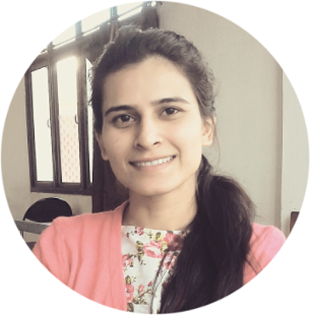
\includegraphics[scale=0.30]{amar.png}
% \section{Father's Name}
 % S. Sukhjinder Singh
 \section{Date of birth}
  12 September, 1991
  \section{Mail}
    \href{mailto:manpreet9112@gmail.com}{\textbf{manpreet9112@}\\gmail.com}
  \section{Tel}
    +91 8872145719
  \section{Git and Web}
    \href{http://github.com/manpreet9112}{\textbf{github.com/manpreet9112}}
    \href{http://manpreet9112.wordpress.com}{\textbf{manpreet9112.\\wordpress.com}}
  \section{Languages}
     \textbf{English}
\includegraphics[scale=0.40]{img/5stars.png}
      \textbf{Hindi}
\includegraphics[scale=0.40]{img/5stars.png}
%      \textbf{Punjabi}
\includegraphics[scale=0.40]{img/5stars.png}
  \section{Programming \\ Language}
    \smartdiagram[bubble diagram]{
        \textbf{WordPress},
       % \textbf{\hspace{1.5mm} WordPress \hspace{1.5mm} \vspace{3mm}},
        \textbf{LaTeX},
        \textbf{HTML}\\\textbf{CSS},
        \textbf{Bash},
        \textbf{PHP},
        \textbf{Python},
       \textbf{SQL},
       \textbf{Mark}\\\textbf{down}
    }
    ~
  \section{Personal Skills}
    \smartdiagram[bubble diagram]{
        %\textbf{Team}\\\textbf{Player},
        \textbf{Curiosity},
        \textbf{Problem}\\\textbf{Solving},
        \textbf{Motivator},
        %\textbf{Logical}\\ {Thinking},
        \textbf{Self}\\ {Learner},
        \textbf{Organize}
    }
    ~
%  \section{Technologies \\ Used}
 %       \textbf{Octave}
  %      \textbf{LaTeX}
   %     \textbf{Django}
    %    \textbf{Python}
     %   \textbf{SageMath}
      %  \textbf{Doxygen}
        %\textbf{Flex}
        %\textbf{Bison}
       % \textbf{GIT}
        %\textbf{GRASS GIS} 
%  ~      
\end{aside}

\section{Objective}
I want to pursue a challenging career with a scope for improvement and
growth. And want to give my best to organisation that I work for.
%stimulating environment that would hone my
%skills and provide me ample opportunities for development in all spheres
%so that I can give
%my best to the organization that I work for.
\section{Education}
\begin{entrylist}
  \entry
    {2013 - 2016}
    {M.C.A}
    {79 \%}
    {Guru Nanak Dev Engineering College, Ludhiana (P.T.U Jalandar)}
  \entry
    {2012}
    {B.C.A}
    {74 \%}
    {Ramgarhia Girls College, Ludhiana (P.U CHD)}
  \entry
    {2009}
    {Higher Secondary Examination}
    {72.36 \%}
    {Govt. girls sen. sec. School,
Ludhiana (PSEB)}
    \entry
    {2007}
    {Matriculation}
    {72.86 \%}
    {Govt. girls sen. sec. School,
Ludhiana (PSEB)}
\end{entrylist}

\section{Projects}
\begin{entrylist}
   \entry
    {}
    {DesignAids}
    {TCC}
    {
       Contribution in DesignAids Project, developed using LaTeX and
SageMath.  
        \textit{\href{https://github.com/manpreet9112/DesignAids}{https://github.com/manpreet9112/DesignAids}}
    }
  \entry
    {}
    {Python-dxf}
    {TCC}
    {
      Build python script to read points from csv, to make footing
design.  
        \textit{\href{https://github.com/manpreet9112/pythondxf}{https://github.com/manpreet9112/pythondxf}}
    }
    \entry
    {}
    {Javascript Graph (Inetractive Graph)}
    {TCC}
    {
       Build Interactive Graph to show Civil data using Javascript and
Amchart library.
        \textit{\href{https://github.com/manpreet9112/JavascriptGraphs}{https://github.com/manpreet9112/JavascriptGraphs}}
    }

  \entry
    {}
    {LibreHatti}
    {TCC}
    {
       Contributed in LibreHatti Project, developed using Python and
Django framework.
        \textit{\href{https://github.com/manpreet9112/LibreHatti}{https://github.com/manpreet9112/LibreHatti}} 
    }
\end{entrylist}
\section{Traineeship Experiences}
\begin{itemize}
\item Semesteral (till-date) Industrial and Software training at Testing
and Consultancy Cell, GNDEC, LDH.
Ludhiana.
\item I am working with Linux from 3 years.
\end{itemize}
\section{Achievements and Certification}
\begin{itemize}
\item Participated in Hactoberfest, 2016 (coding competition).
\item Executive member of Linux User Group, GNDEC, Ludhiana.
\item Volunteer Certificate from workshop “Producing Elegant Technical
Research Reports Efficiently” using
LaTeX at TCC, GNDEC, Ludhiana in 2016.
\item Co-organized and Volunteered LaTeX workshop at Chitkara
University, Rajpura in 2016.
\end{itemize}
\end{document}
